\part{Lösungsansatz}
\label{part:solution}
\begin{frame}[fragile]{}
	\textit{Erweiternde Darstellungen erstellen und räumlich wie zeitlich in den Versuch integrieren}
	\pause
	\begin{itemize}
		\item Nicht sichtbare, physikalische Eigenschaften im Raum darstellen
		\begin{itemize}[topsep=-5px]
			\setlength{\itemsep}{-5px}
			\item Magnetfelder durch Feldlinien und Vektoren
			\item Stromfluss, Messwerte und ideale Kompassnadel 
		\end{itemize}
		\pause
		\item Positionierung und Stabilisierung der HoloLens nutzen		
		\item Echtzeitdaten (Messwerte) an die HoloLens übermitteln und darstellen
		\item Technische Einschränkungen beim Design berücksichtigen
	%	\begin{itemize}[topsep=-5px]
	%		\setlength{\itemsep}{-5px}
	%		\item Maßnahmen zur Vermeidung von Problemen anwenden
	%		\item Angepasstes Design
	%		\item Vorgefertigte Objekte nutzen
	%	\end{itemize}
		\item Anpassung von realen Objekten, um Integration mit der Anwendung zu verbessern
	\end{itemize}
\end{frame}

\begin{frame}[fragile]{}
	\vspace{-10px}
	\begin{minipage}{0.25\textwidth}
		{\setstretch{1.0}
			\begin{itemize}[itemsep=1mm]
				\item Feldlinien
				\item Kompass-Skala
				\item Virtuelle Nadel
				\item Stromrichtung
				\item Plus \& Minus
				\item Messwerte
			\end{itemize}
		}
	\end{minipage}
	\begin{minipage}{0.7\textwidth}
		\centering
		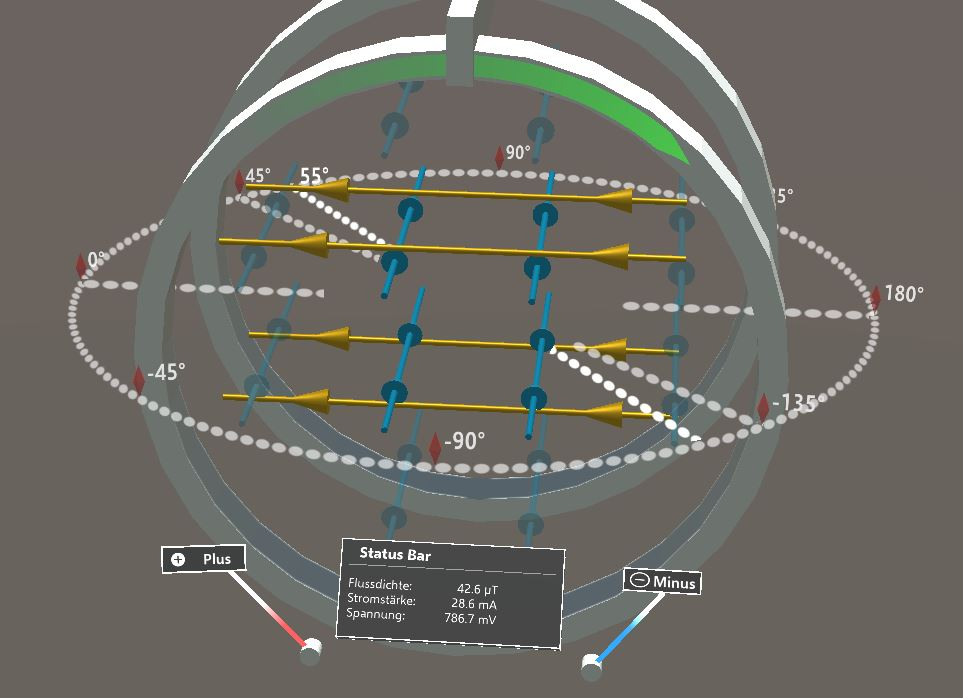
\includegraphics[width=0.95\textwidth]{images/unity/overview.jpg}\\
		\scriptsize Darstellungen in der Entwicklungsumgebung (Unity). Auflösung und Qualitätseinstellungen entsprechen den Werten auf der HoloLens.
	\end{minipage}
\end{frame}

\begin{frame}[fragile]{}
\begin{figure}
	\vspace{-10px}
	\centering
	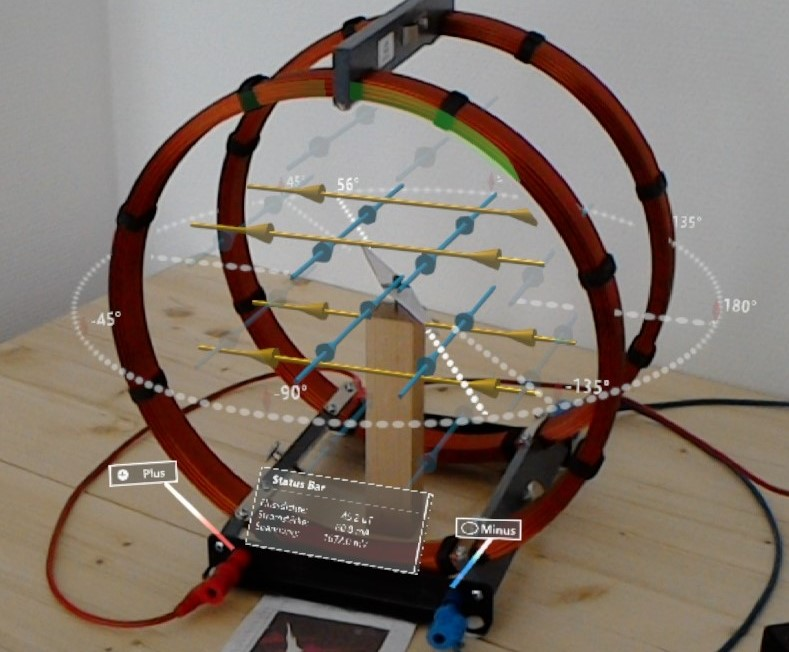
\includegraphics[width=0.7\textwidth]{images/HL/fieldlines_cut.jpg}\\
	\scriptsize Screenshot von der HoloLens mit Feldliniendarstellung.
\end{figure}
\end{frame}

\begin{frame}[fragile]{}
\begin{figure}
	\vspace{-10px}
	\centering
	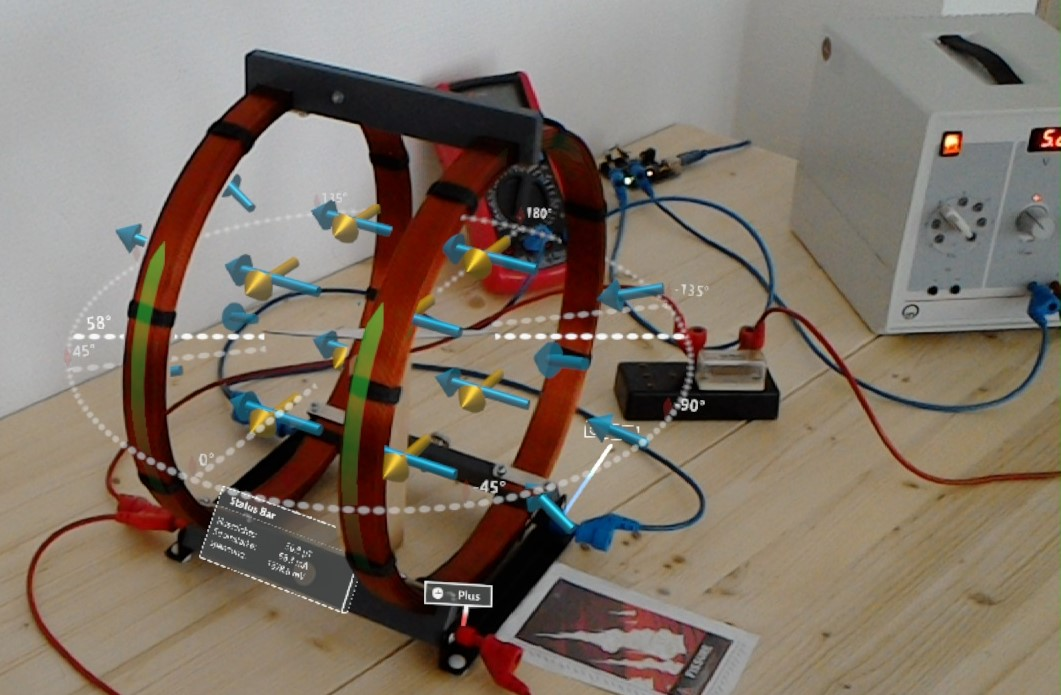
\includegraphics[width=0.85\textwidth]{images/HL/Vektoren.jpg}\\
	\scriptsize Screenshot von der HoloLens mit Vektordarstellung.
\end{figure}
\end{frame}

\begin{frame}[fragile]{Near Plane Fading}
\begin{figure}
	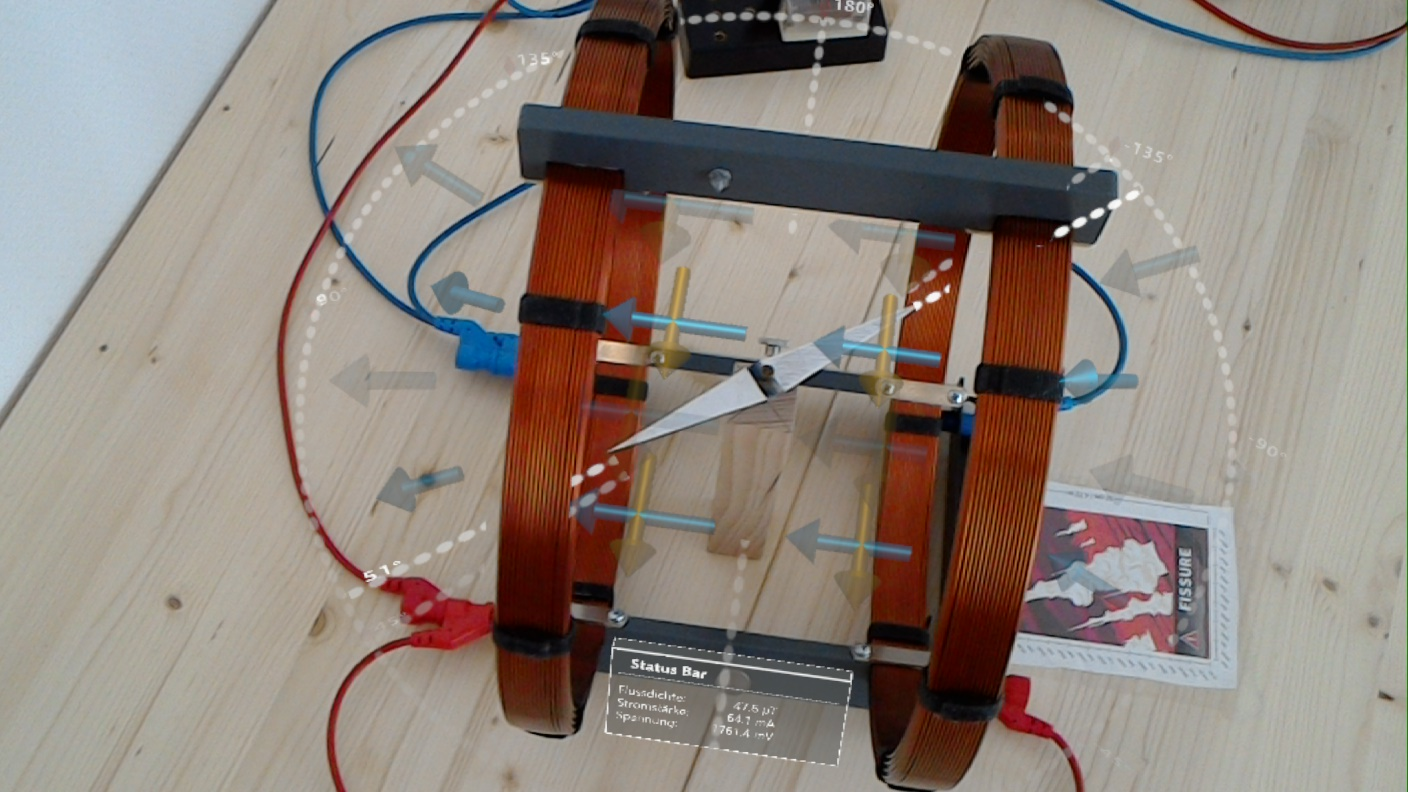
\includegraphics[width=0.8\textwidth]{images/HL/compass.jpg}
\end{figure}
\end{frame}

\begin{frame}[fragile]{Design}
\begin{itemize}
	\item Nutzung etablierter Darstellungsmodelle
	\pause
	\item Anwendung für Nutzung im Abstand von ca. 1,3 m designet, zu nah liegende Objekte werden ausgeblendet
	\begin{itemize}
		\item Hologramme passen ins Sichtfeld, sind nicht zu dicht positioniert, nutzen Screenspace aus, Komfortable Nutzung möglich
	\end{itemize}
	\pause
	\item 
	\pause
	\item Umsetzung empfohlener Maßnahmen zur Verbesserung der Performance
\end{itemize}
\end{frame}


\part{Ergebnisse}
\label{part:results}
\begin{frame}[fragile]{Dargestellte Informationen}
\begin{itemize}
	\item Visualisierung der Komponenten des Magnetfeldes in zwei Darstellungen und in Echtzeit
	\item Darstellung einer vorberechneten Lösung für eine ausgewählte Ebene des Feldes der Spule
	\item Kennzeichnung der Stromrichtung
	\item Integration einer virtuellen Kompass-Skala mit Hervorhebung wichtiger Zustände
	\item Einbettung einer virtuellen Kompassnadel auf Basis theoretischer Werte
	\item Numerische Darstellung gemessener und berechneter Echtzeitdaten
\end{itemize}
\end{frame}

\begin{frame}[fragile]{Technische Bewertung}

\setlength\extrarowheight{1pt}
\def\arraystretch{1.1}
\begin{table}
	\centering
	\begin{tabular}{l{5cm}|l}
		Kriterium & Bewertung \\
		\hline
		\hline
		Framerate & Optimal\\
		\hline
		Stabilität & Fast optimal\\
		\hline
		Positionierung & Fast optimal\\
		\hline
		Komfortzone & Optimal\\
		\hline
		Tiefen Wechsel & Fast optimal\\
		\hline
		FoV-Grenzen & Optimal\\
		\hline
		Input Interaction Clarity & Erfüllt\\
		\hline
		Anpassung an Nutzerposition & Optimal\\
	\end{tabular}
\end{table}
\scriptsize Bewertung anhand von Qualitätskriterien der Dokumentation. Stufen: ''Optimal'', ''Erfüllt'' und ''Nicht erfüllt''.
\end{frame}


\part{Ausblick}
\label{part:future}
\begin{frame}[fragile]{Erweiterungen}
\usebeamerfont{frametitle}\textcolor{blue}{Inhaltlich:} \usebeamerfont{text}\textit{Weitere Lerninhalte integrieren}
\begin{itemize}
	\item Weitere Inhalte, z.B. Rechte-Hand-Regel
	\item Weitere Experimente, z.B. Ablenkung eines Elektronenstrahles
\end{itemize}
\pause
\vskip 1em
\usebeamerfont{frametitle}\textcolor{blue}{Technisch:} \usebeamerfont{text}\textit{Portierung für HoloLens 2}
\begin{itemize}
	\item Auflösung x4 pro Auge, Sichtfeld x2 (Fläche)
	\item Tragekomfort und Interaktion verbessert
\end{itemize}

\vspace{50px}
\end{frame}



\part{Diskussion}
\begin{frame}[fragile]{}
Vielen Dank für Ihre Aufmerksamkeit!

\vspace{1em}
\hspace{1em} Fragen?
\end{frame}
